%!TEX root = kotov.tex
\section{Task 2: автобусы}

\begin{task}
    Предположим, что вы приезжаете в новый город и видите автобус с номером 100. Требуется с помощью байесовского подхода оценить общее количество автобусных маршрутов в городе. Каким априорным распределением стоит воспользоваться (обоснуйте выбор его параметров)? Какая из статистик апостериорного распределения будет наиболее адекватной (обоснуйте свой выбор)? Как изменятся оценки на количество автобусных маршрутов при последующем наблюдении автобусов с номерами 50 и 150?
    \textit{Подсказка: воспользоваться результатами предыдущей задачи. При этом обдумать как применить непрерывное распределение к дискретным автобусам.}
\end{task}

\begin{solution}
    Номера автобусов --- дискретная величина. Будем моделировать их непрерывным распределением $U[0, \theta]$ так, что под номером будет понимать $\lceil x \rceil$, где $x \sim U[0, \theta]$, т.е. целая часть сверху случайной величины. Этот выбор кажется разумным, так как у нас нет знания о частоте хождения автобусов или отношения кол-во автобусов на маршруте к общему числу автобусов, т.е. в такой модели мы предполагаем, что можем наблюдать любой номер автобуса равновероятно.

    Нам надо оценить $\theta$, которая может быть, в принципе, любым положительным целым числом. Здесь сделаем еще одно предположение: номера автобусов считаем заданными подряд с 1, т.е. если у нас всего 3 автобуса в атвопарке, то их номера будут $1, 2, 3$, а не $1, 5, 10$ или $4, 5, 6$, так сказать, предположение здравого смысла.

    В качестве априорного распределения возьмем распределение Парето:
    \begin{equation}
        p(\theta | \alpha, \beta) = \frac{\alpha \beta^{\alpha}}{\theta^{\alpha + 1}}[\theta \ge \beta],
    \end{equation}
    причем в качестве $\alpha$ и $\beta$ можно выбрать исходя их каких-то знаний об автопарке города.
    Так, например, если мы пронаблюдали автобус с номером 100, то $\beta=100$, если изначально $\beta < 100$, т.к. мы точно знаем, что такой номер автобуса существует. Для дальнейшего будем считать, что $\beta = 100$.

    Теперь мы наблюдаем еще один автобус, но с номером 150. Тогда $\beta$ еще подправится и станет равной 150, что значит, что значения $\theta > 150$ теперь тоже стали более вероятными. Однако, если мы пронаблюдали еще и автобус с номером 50, то распределение деформируется так, что небольшие $\theta$ станут более вероятными, а большие наоборот --- менее, это хорошо видно из следующей картинки, т.к. в этом случае у нас просто увеличилась $\alpha$ на 1:
    \begin{figure}[H]
        \centering
        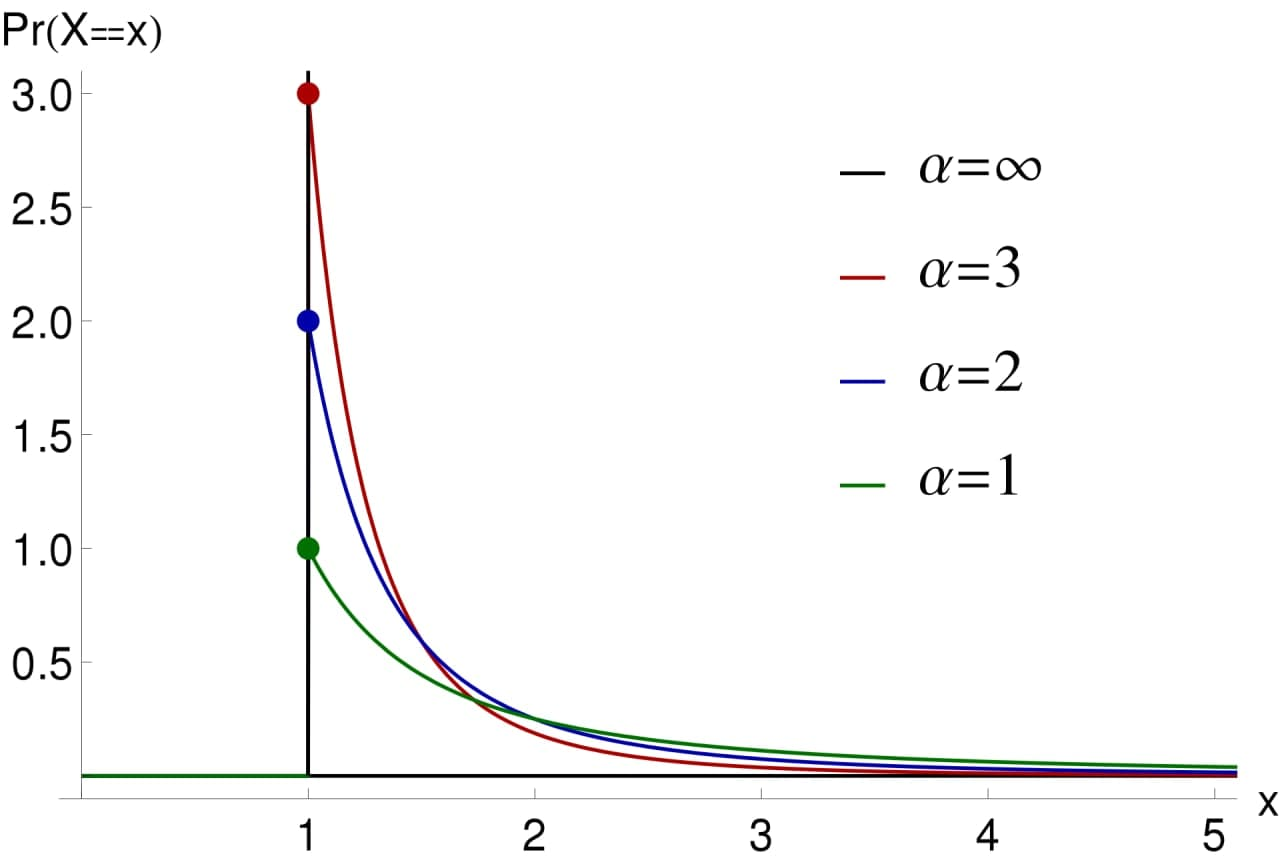
\includegraphics[width=0.6\textwidth]{pics/pareto.jpg}
        \caption{Распределения Парето с различными $\alpha$ при $\beta = 1$}
    \end{figure}
    Видно, что хвост поджимается при увеличении $\alpha$

    Как мы видели из предыдущей задачи, мода распределения есть $\beta$. В целом, норм статистика, но понятно, что грубая, так, например, если у нас действительно всего 150 маршрутов, то все окей, но это все равно, что оценивать количество маршрутов по наибольшему наблюдаемому номеру автобуса\ldots

    Посмотрим на среднее и медиану:
    \begin{gather}
        \braket{\theta} = \frac{\alpha \beta}{\alpha - 1} \\
        \theta_m = \beta \sqrt[\alpha]{2}
    \end{gather}

    Обе эти статистики завысят оценку $\theta$ по сравнению с модой, к тому же здесь используется наше априорное знание, в отличии от моды. Какое именно выбрать из эти двух? Сложно сказать. По классике я бы выбирал среднее, но против медианы ничего, на первый взгляд, сказать не могу противного. Среднее среди всех трех будет наибольшей, при этом в пределе $\alpha \to +\infty$, все три статистики стремятся к $\beta$.

\end{solution}
